% !TeX TS-program = xelatex
\documentclass[12pt]{article}
%\usepackage[utf8]{inputenc}
\usepackage{indentfirst}
\usepackage{float}
\usepackage{array}
\usepackage{url}
\urlstyle{tt}
\usepackage{enumitem, amsmath, amssymb, amsfonts, latexsym, mathrsfs}
\usepackage{graphicx}
\usepackage{subfig}
\usepackage{multicol}
\usepackage{booktabs}
\usepackage{ragged2e}
\usepackage{svg}
\usepackage{xcolor}
\usepackage{tabularray}
\usepackage{listings}
\usepackage{atkinson} %% Option 'sfdefault' if the base
%% font of the document is to be sans serif.
\usepackage[T1]{fontenc}
\setmainfont{Atkinson Hyperlegible}
\renewcommand{\familydefault}{\sfdefault}

\usepackage[spanish]{babel}

\usepackage[backend=biber]{biblatex}
\bibliography{referencias}
\usepackage{csquotes}
%New colors defined belowd
\usepackage{}
\definecolor{codegreen}{rgb}{0,0.6,0}
\definecolor{codegray}{rgb}{0.5,0.5,0.5}
\definecolor{codepurple}{rgb}{0.58,0,0.82}
\definecolor{backcolour}{rgb}{0.95,0.95,0.92}
\lstdefinestyle{mystyle}{
  backgroundcolor=\color{backcolour},   commentstyle=\color{codegreen},
  keywordstyle=\color{magenta},
  numberstyle=\tiny\color{codegray},
  stringstyle=\color{codepurple},
  basicstyle=\ttfamily\footnotesize,
  breakatwhitespace=false,
  breaklines=true,
  captionpos=b,
  keepspaces=true,
  numbers=left,
  numbersep=5pt,
  showspaces=false,
  showstringspaces=false,
  showtabs=false,
  tabsize=2
}
%"mystyle" code listing set
\lstset{style=mystyle}
%\lstset{basicstyle=\ttfamily\footnotesize,breaklines=true}

\usepackage{notoccite}

\usepackage{multicol}
\setlength{\columnseprule}{1pt}
\def\columnseprulecolor{\color{black}}





\date{}
% Comand para keywords
\providecommand{\keywords}[1]
{
  \small
  \textbf{\textit{Keywords---}} #1
}

% Tipografía
%\usepackage{helvet}
%\renewcommand{\familydefault}{\sfdefault}
%\usepackage[sfdefault]{Chivo}
%\usepackage{comment}


\urlstyle{same}
% \tolerance=9999
% \emergencystretch=10pt
\hyphenpenalty=10000
\sloppy
% \exhyphenpenalty=100

\renewcommand{\figurename}{\textbf{Figura.}}
\renewcommand\spanishtablename{Tabla.}

% Interlineado
\usepackage{setspace}
\spacing{1.15}

% Márgenes
\usepackage[a4paper]{geometry}
\geometry{top=2.5cm, bottom=2.5cm, left=2cm, right=2cm}

% Número de página
\usepackage{fancyhdr}
\pagestyle{fancy}
\rhead[]{}
\lhead[]{}
\renewcommand{\headrulewidth}{0pt}
\rfoot[]{\thepage}
\cfoot[]{}

\usepackage[breaklinks]{hyperref}
% Setup de hiperenlaces
\hypersetup{
    colorlinks=true,
    linkcolor=blue,
    filecolor=magenta,
    urlcolor=cyan,
    pdftitle={Arquitectura de las consolas de videojuegos},
    pdfpagemode=FullScreen,
    citecolor = green
    }
\usepackage[norule]{footmisc}

%_____________________________________________________________________________
%_____________________________________________________________________________
%_____________________________________________________________________________
%_____________________________________________________________________________
\hbadness=50000
\usepackage{microtype}
\begin{document}
\nocite{atkinson}
\nocite{circuitverse}
\nocite{chatgpt}
\nocite{duke}
\nocite{texstudio}
% PORTADA
\begin{titlepage}
        \begin{center}


        \hrule
        \vspace{1cm}
        %{\bfseries\Large UNIVERSIDAT JAUME I \par}
        \vspace{1cm}
        {\bfseries\huge Apuntes de Consolas y Dispositivos de Videojuegos \par}
        \vspace{2cm}

        \begin{figure}[H]
            \centering
            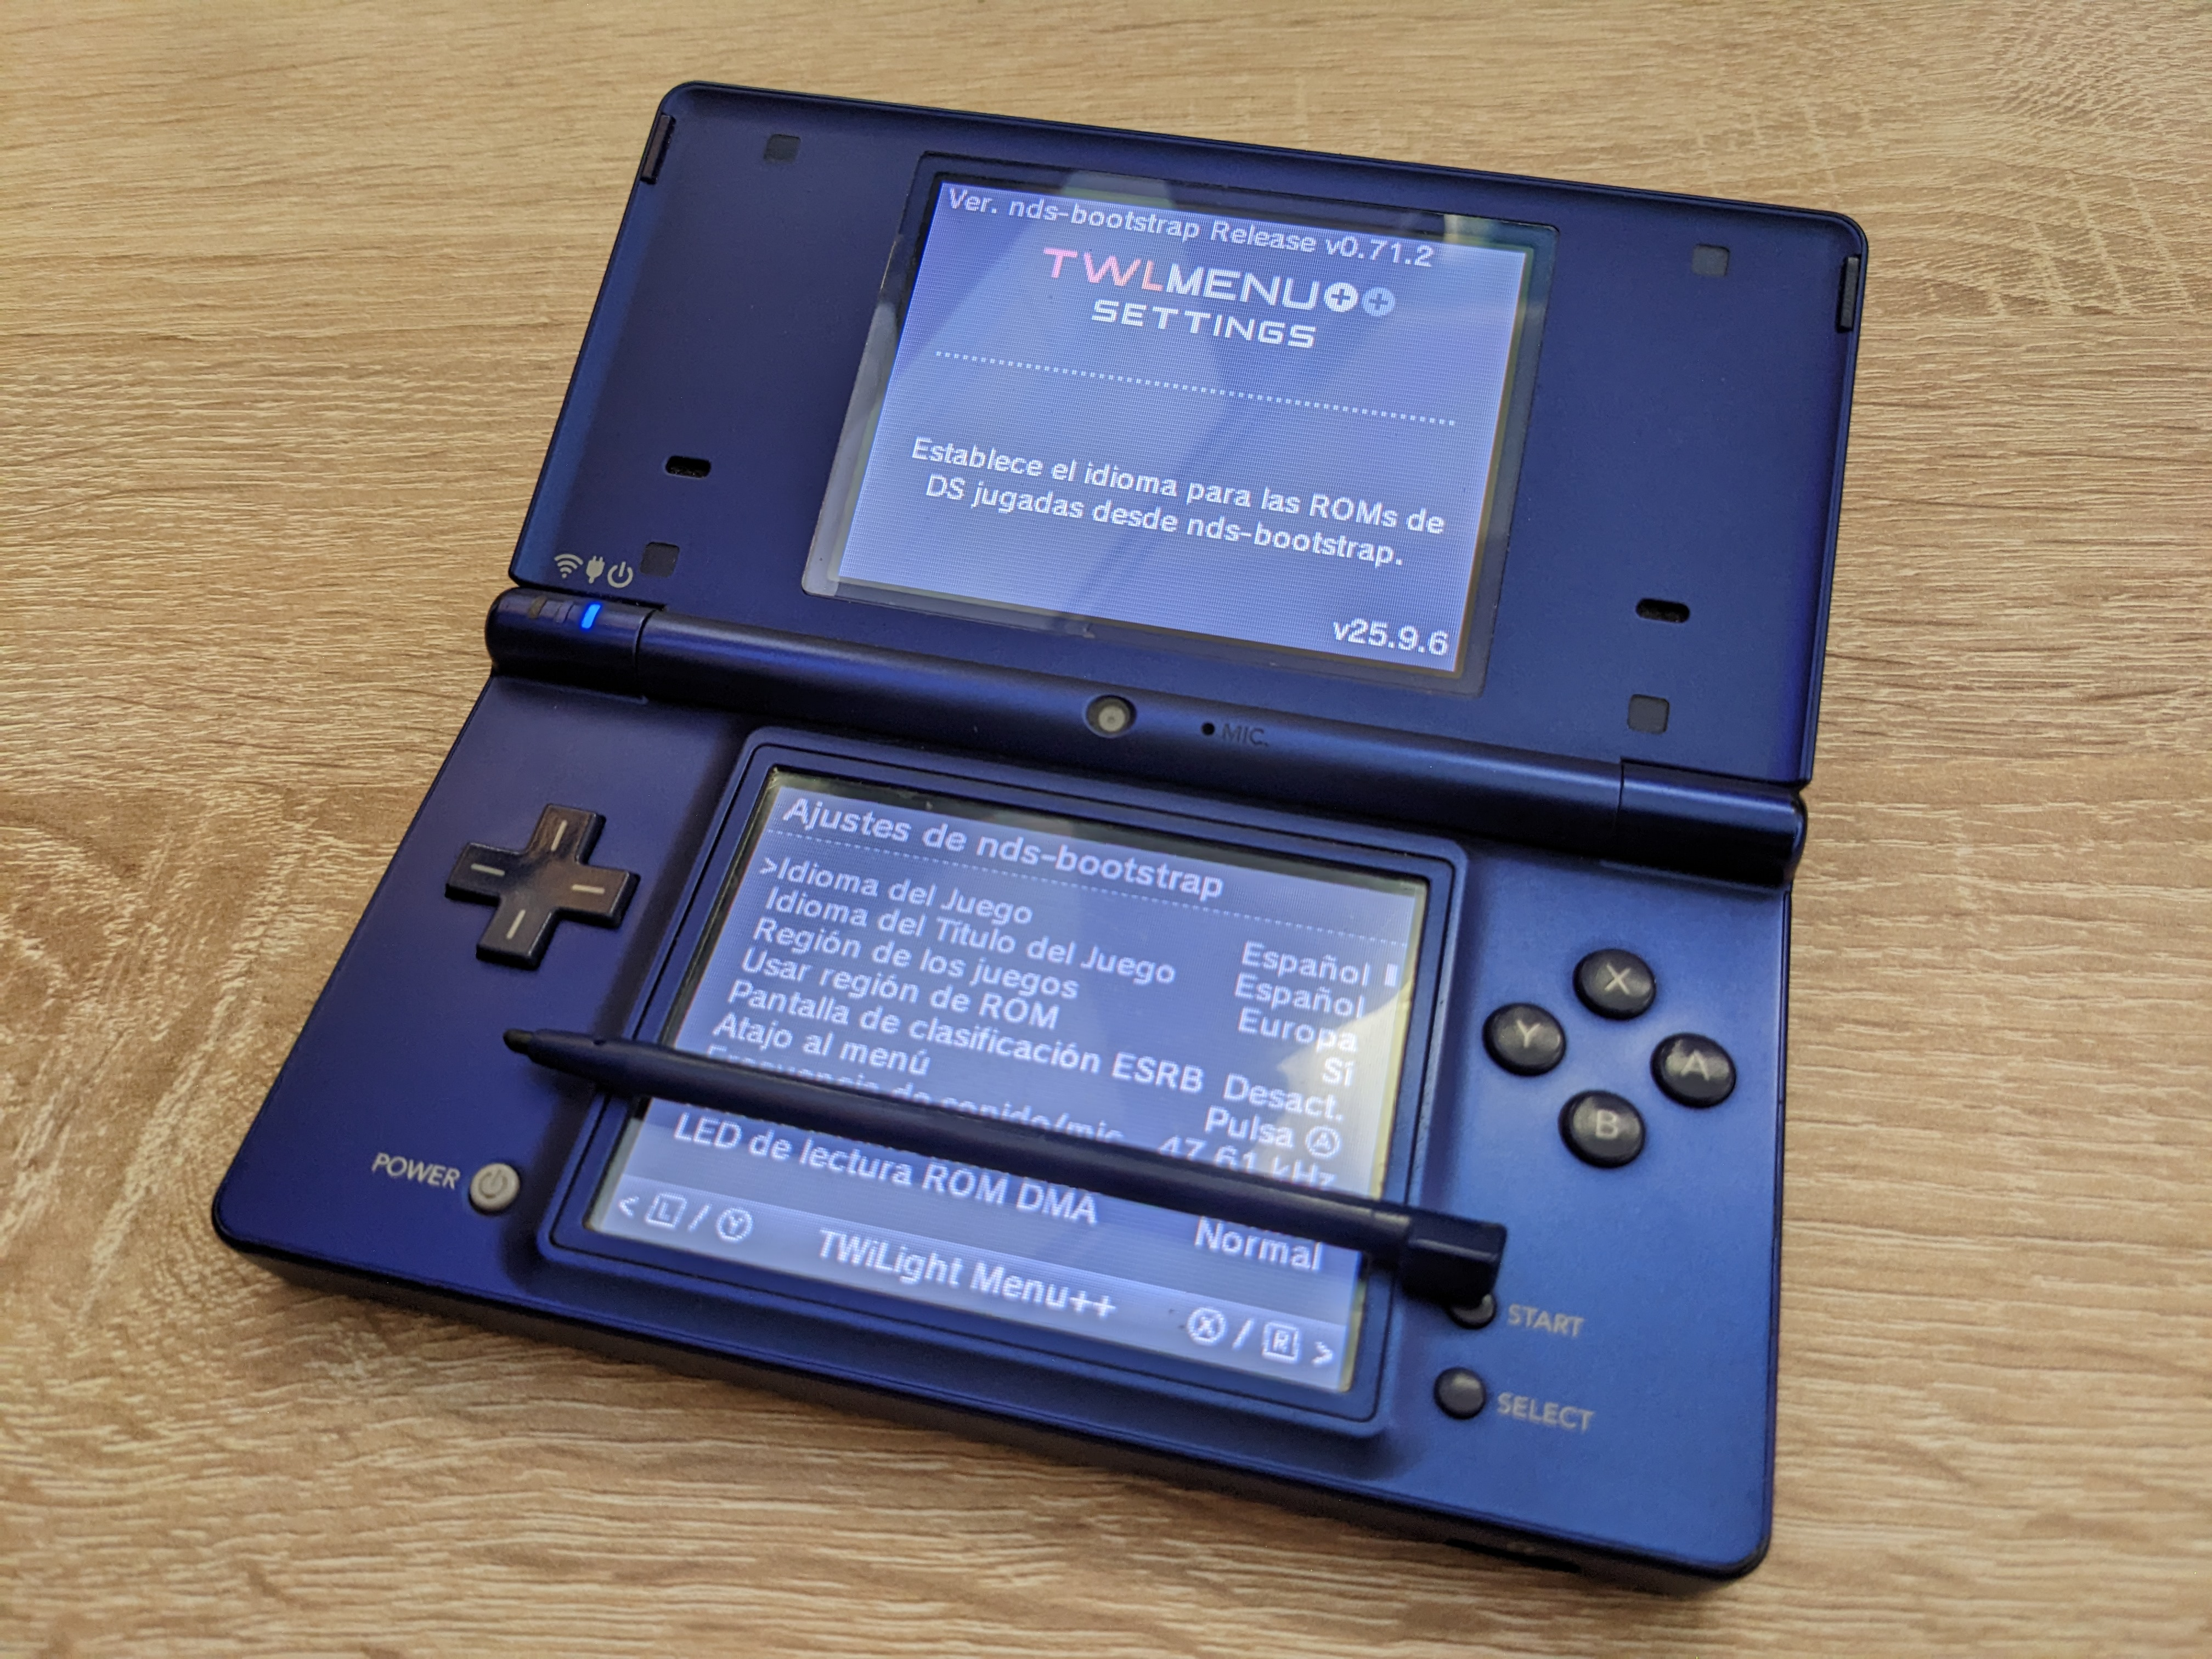
\includegraphics[width=\textwidth]{dsi.jpg}
            \caption*{\footnotesize{\textit{Nintendo DSi con Homebrew y emulador de NDS}}}
            \label{fig:dsi}
        \end{figure}

        {\large
        Jesús Jiménez Montero \\
        \par}
        \vspace{1cm}
        \hrule
        \vspace{1cm}

        {\large
        \textit{Versión 5: Registros y RAM\\
        \today}
        \par}
        \end{center}
\end{titlepage}

% ÍNDICE
%\renewcommand{\tableofcontents}{Indice general}
\newpage
\renewcommand{\contentsname}{Tabla de contenidos}
\setcounter{secnumdepth}{5}
\tableofcontents
\setcounter{tocdepth}{4}

\newpage
%-----------------------------------------------------------------
%-----------------------------------------------------------------
% Tabla de figuras
\newpage
\renewcommand{\listfigurename}{Lista de figuras}
\thispagestyle{empty}
\listoffigures
\newpage

\renewcommand{\listtablename}{Lista de tablas}
\listoftables
\newpage

%-----------------------------------------------------------------
%-----------------------------------------------------------------

%%%%%%%%%%%%%%%%%%%%%%%%%%%%%%%%%%%%%%%%%%%%%%%%%%%%%%%%%%%%%%%%%%%%%%%%%%
%%%%%%%%%%%%%%%%%%%%%%%%%%%%%%%%%%%%%%%%%%%%%%%%%%%%%%%%%%%%%%%%%%%%%%%%%%
\section{Registro de 1bit}
	\subsection{Tabla de verdad y explicación del circuito}

		El registro de 1bit se compone de dos piezas fundamentales, el \textit{data flip flop} (DFF) y un MUX que sirve como el selector de escritura o lectura.
		Esta pieza sirve para almacenar (o recordar \cite{nisan_nand2tetris_2005}) un valor durante un tiempo.
		% \usepackage{tabularray}
		\begin{table}[H]
			\centering
			\caption{Tabla de verdad de registro de 1bit \cite{chatgpt}}
			\label{tab:1bit}
			\begin{tblr}{
					width = \linewidth,
					colspec = {Q[198]Q[183]Q[475]},
					cells = {c, font=\ttfamily},
					hline{1,5} = {-}{0.08em},
				}
				\textbf{Load} & \textbf{Data} & \textbf{Q (next state)}\\
				0 & X & Q (no change)\\
				1 & 0 & 0\\
				1 & 1 & 1
			\end{tblr}
		\end{table}
	\subsection{Esquema del circuito exterior y exterior}
		\begin{figure}[H]
			\centering
			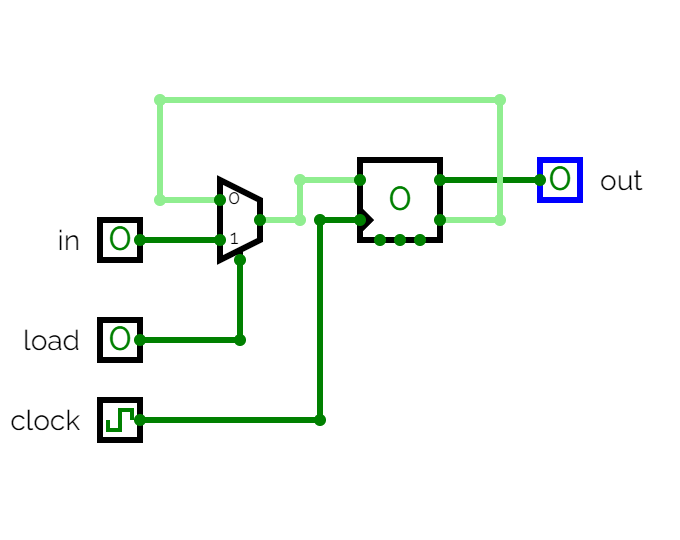
\includegraphics[width=0.75\linewidth]{RAM/REG1Bit.png}
			\caption{Esquema interior de un registro de 1 bit.}
			\label{fig:reg1bit}
		\end{figure}
	\subsection{Implementación HDL}
		\begin{figure}[H]
			\centering
			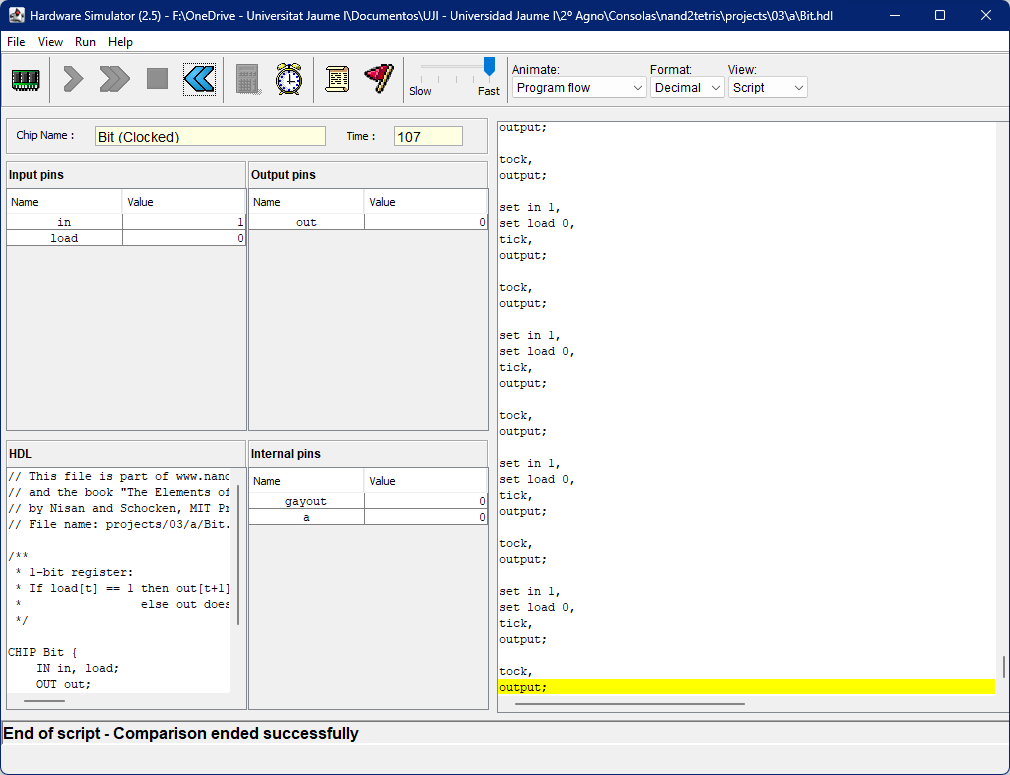
\includegraphics[width=0.75\linewidth]{RAM/bit_hdl}
			\caption{Implementación en Hardware Simulator de Registro de 1bit}
			\label{fig:bithdl}
		\end{figure}
		\subsubsection{Archivo .HDL}
			\begin{lstlisting}
	CHIP Bit {
		IN in, load;
		OUT out;

		PARTS:
		Mux(a=gayout,b=in,sel=load,out=a);
		DFF(in=a,out=out,out=gayout);
	}
			\end{lstlisting}

\newpage
%%%%%%%%%%%%%%%%%%%%%%%%%%%%%%%%%%%%%%%%%%%%%%%%%%%%%%%%%%%%%%%%%%%%%%%%%%
%%%%%%%%%%%%%%%%%%%%%%%%%%%%%%%%%%%%%%%%%%%%%%%%%%%%%%%%%%%%%%%%%%%%%%%%%%
\section{REG16}
	\subsection{Tabla de verdad y explicación del circuito}
		Un registro de 16bit se crea mediante la conjunción de varios (16 en concreto) registros de 1bit.

		\begin{table}[H]
			\centering
			\caption{Tabla de verdad registro de 16Bit  \cite{chatgpt}}
			\label{tab:fulladder}
			\begin{tblr}{
					width = \linewidth,
					colspec = {Q[112]Q[402]Q[402]},
					row{even} = {c},
					row{1} = {c},
					row{3} = {c},
					row{5} = {c},
					row{7} = {c},
					row{9} = {c},
					cell{11}{1} = {c},
					cell{11}{2} = {c},
					cell{11}{3} = {c},
					hline{1,13} = {-}{0.08em},
					cells = {font=\ttfamily},
				}
				\textbf{Load} & \textbf{Data[15:0]} & \textbf{Q[15:0] (next state)}\\
				0 & X & Q[15:0] (no change)\\
				1 & 0000 0000 0000 0000 & 0000 0000 0000 0000\\
				1 & 0000 0000 0000 0001 & 0000 0000 0000 0001\\
				1 & 0000 0000 0000 0010 & 0000 0000 0000 0010\\
				1 & 0000 0000 0000 0011 & 0000 0000 0000 0011\\
				1 & 0000 0000 0000 0100 & 0000 0000 0000 0100\\
				1 & 0000 0000 0000 0101 & 0000 0000 0000 0101\\
				1 & 0000 0000 0000 0110 & 0000 0000 0000 0110\\
				1 & 0000 0000 0000 0111 & 0000 0000 0000 0111\\
				... & ...               &       ...          \\
				1 & 1111 1111 1111 1111 & 1111 1111 1111 1111
			\end{tblr}
		\end{table}
	\subsection{Esquema del circuito exterior y exterior}
		\begin{figure}[H]
			\centering
			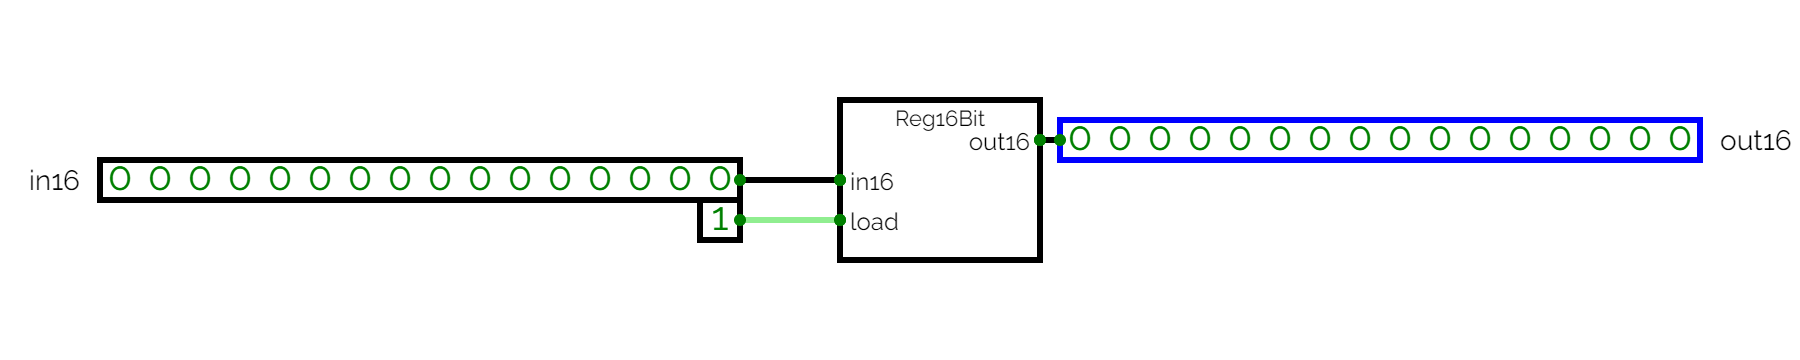
\includegraphics[width=0.75\linewidth]{RAM/REG16bit_ext}
			\caption{Circuito externo de REG16}
			\label{fig:reg16bitext}
		\end{figure}

		\begin{figure}[H]
			\centering
			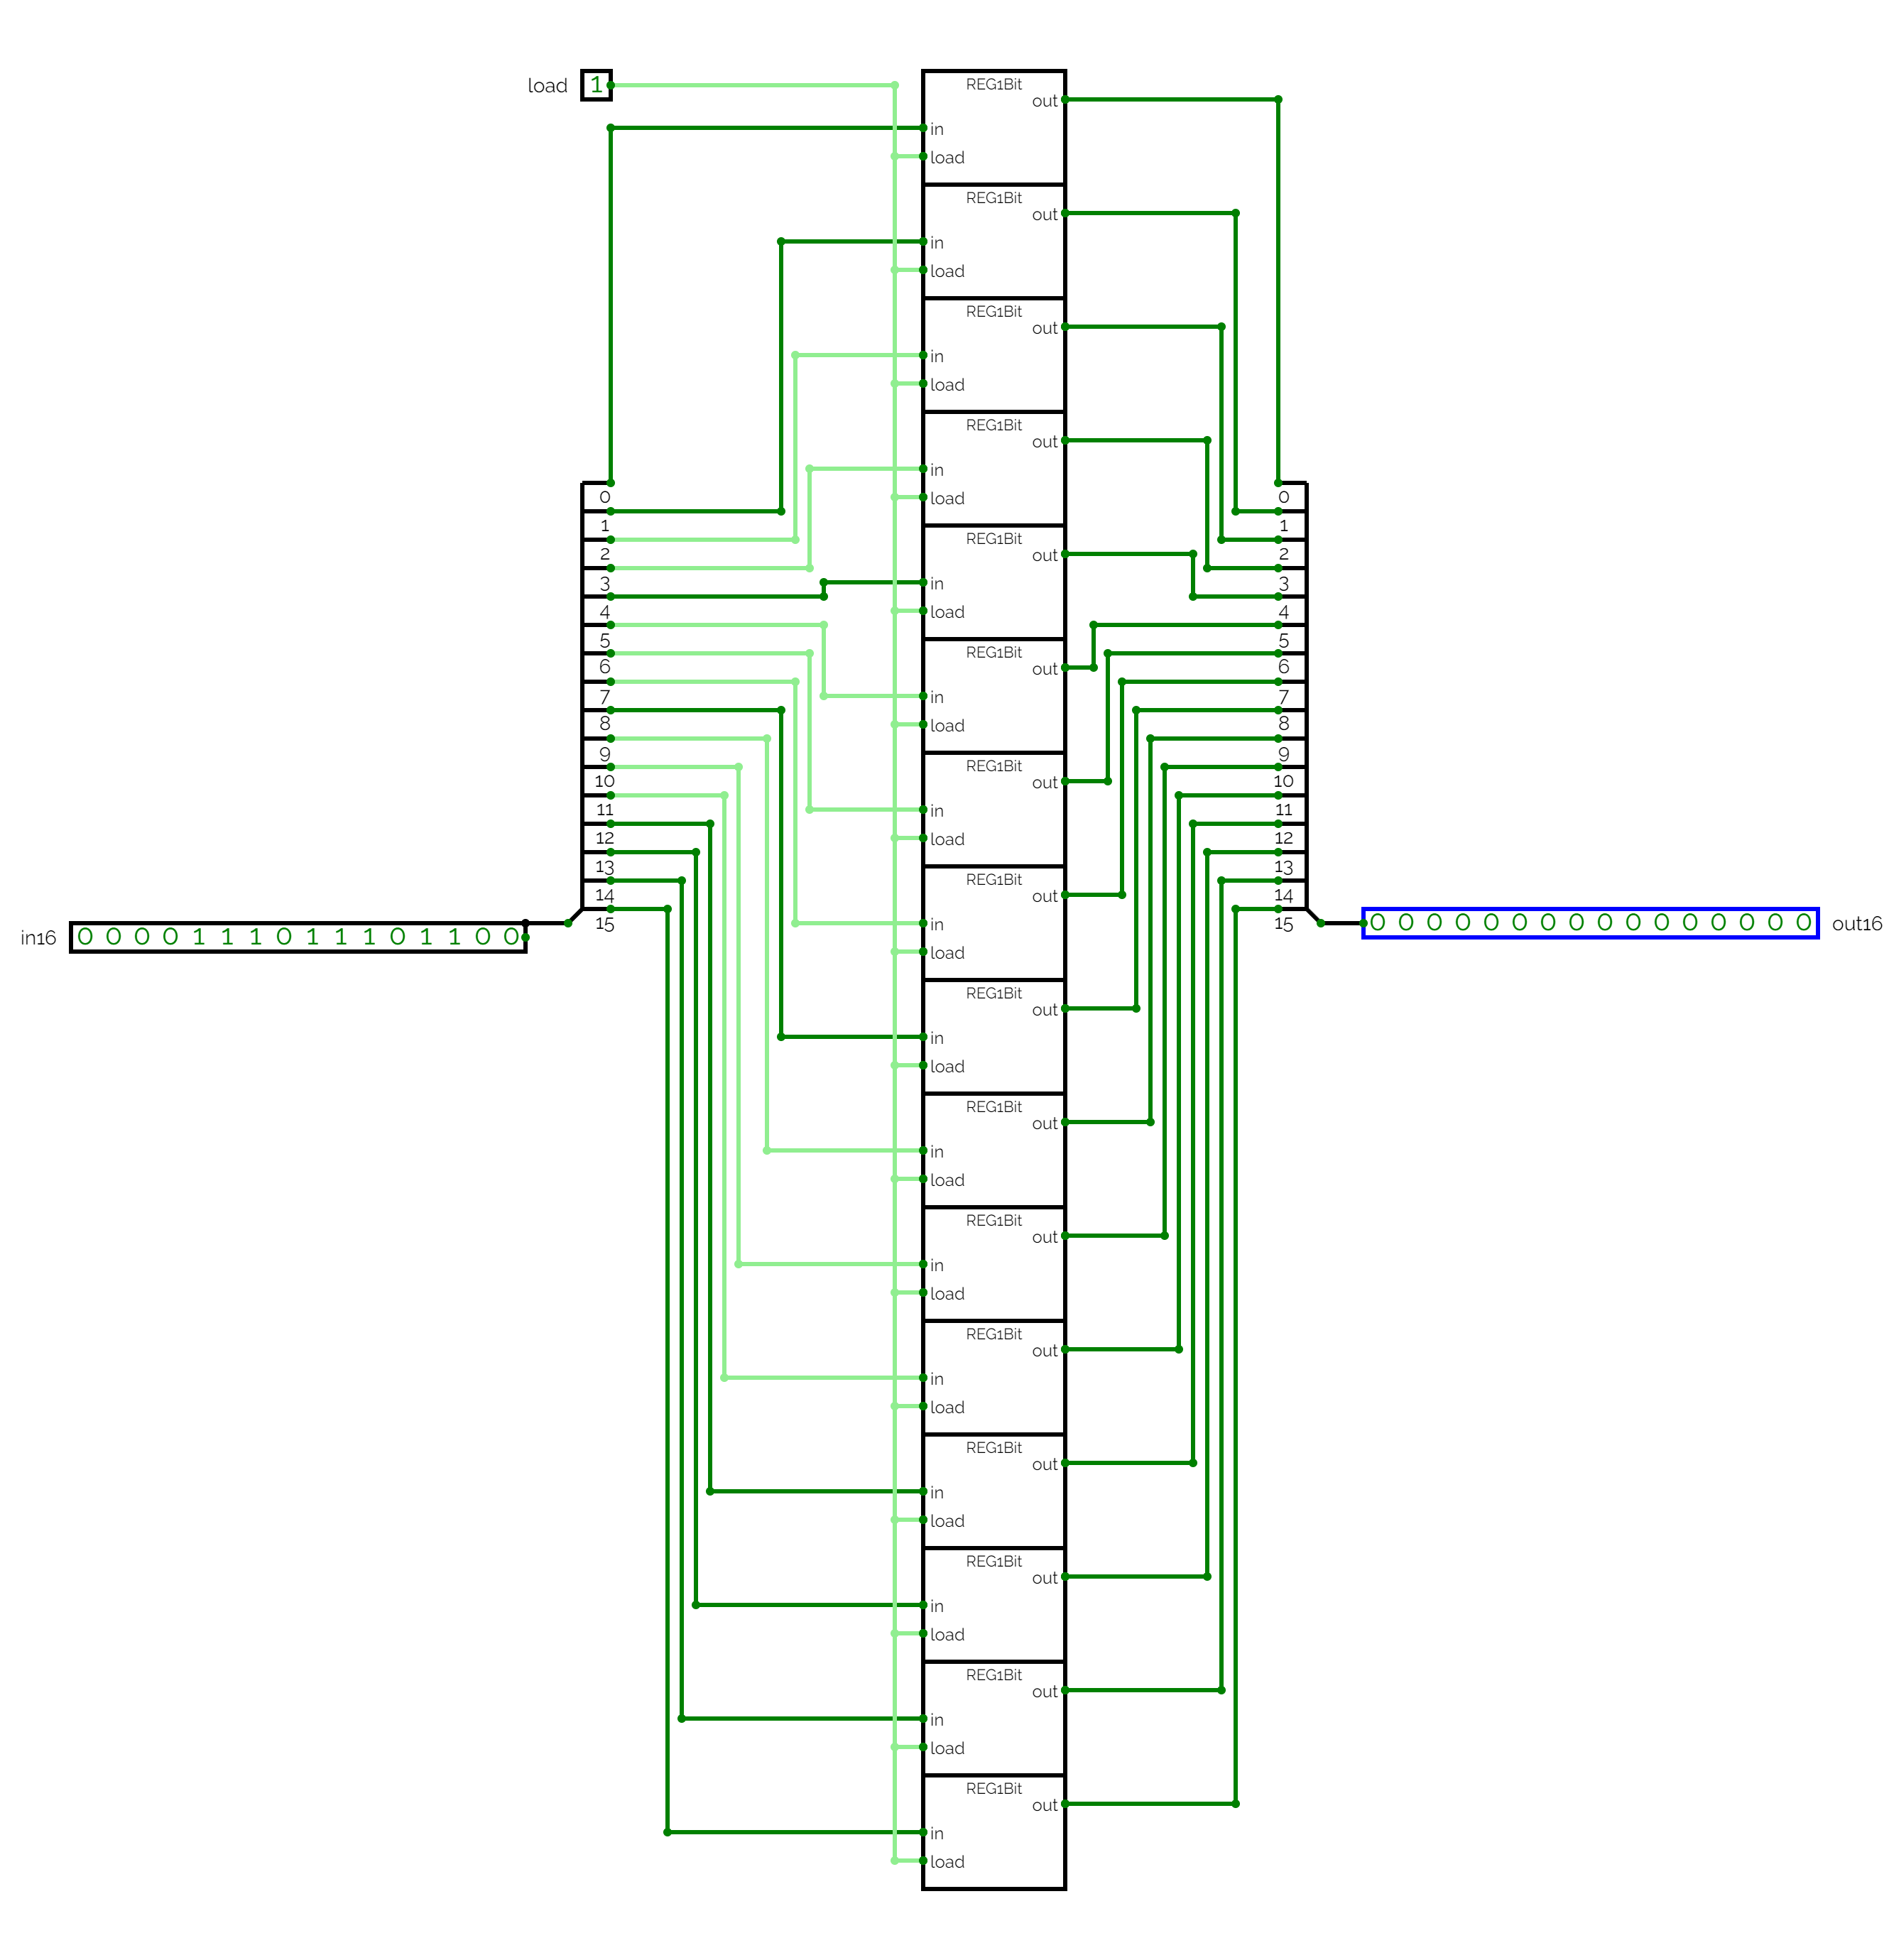
\includegraphics[width=0.75\linewidth]{RAM/Reg16Bit}
			\caption{Circuito interno de REG16}
			\label{fig:reg16bit}
		\end{figure}

	\subsection{Implementación HDL}
		\begin{figure}[H]
			\centering
			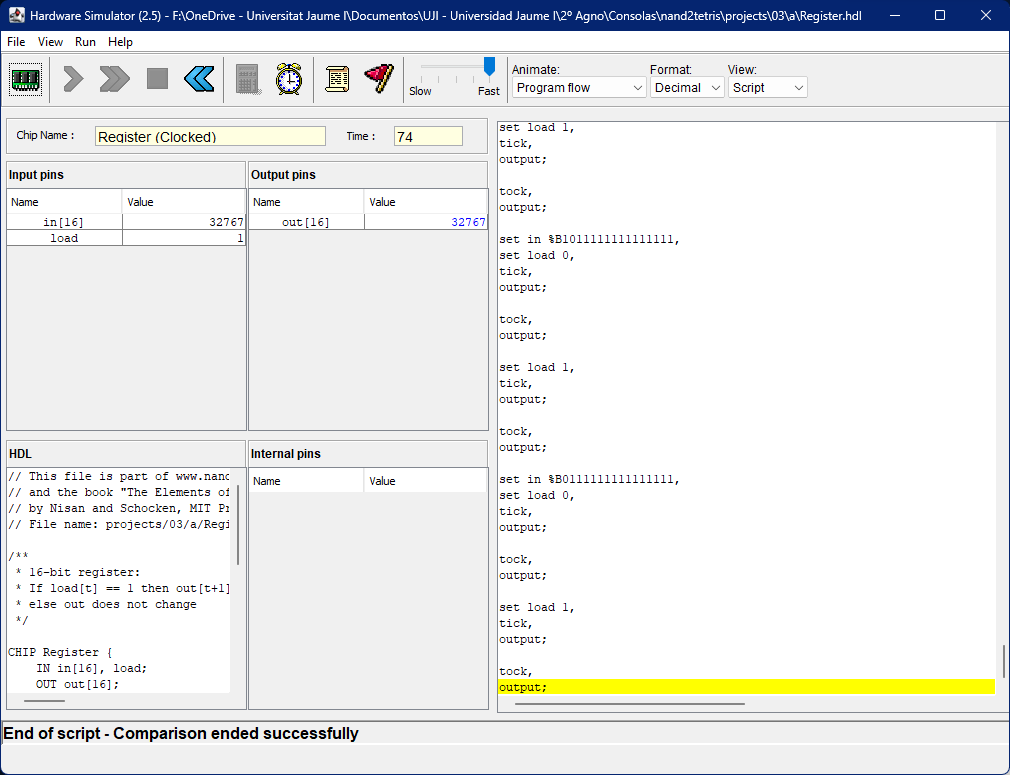
\includegraphics[width=0.75\linewidth]{RAM/reg_hdl}
			\caption{Implementación en Hardware Simulator de REG16}
			\label{fig:reghdl}
		\end{figure}

		\subsubsection{Archivo .HDL}
			\begin{lstlisting}
				CHIP Bit {
					IN in, load;
					OUT out;

					PARTS:
					Mux(a=gayout,b=in,sel=load,out=a);
					DFF(in=a,out=out,out=gayout);
				}
			\end{lstlisting}

\newpage
%%%%%%%%%%%%%%%%%%%%%%%%%%%%%%%%%%%%%%%%%%%%%%%%%%%%%%%%%%%%%%%%%%%%%%%%%%
%%%%%%%%%%%%%%%%%%%%%%%%%%%%%%%%%%%%%%%%%%%%%%%%%%%%%%%%%%%%%%%%%%%%%%%%%%
\section{RAM8}
\subsection{Tabla de verdad y explicación del circuito}
Una RAM es un conjunto de registros n y w-bit, siendo n la cantidad de registros y w la cantidad de bits por registro.
La RAM8 se compone de 8 registros, o de 2 RAM4.
	\begin{table}[H]
		\centering
		\caption{Tabla de verdad registro de 16Bit \cite{chatgpt}}
		\label{tab:ram8}
		\begin{tblr}{
				width = \linewidth,
				colspec = {Q[88]Q[204]Q[315]Q[323]},
				cells = {c, font=\ttfamily},
				hline{1,11} = {-}{0.08em},
			}
			\textbf{Load} & \textbf{Address[2:0]} & \textbf{In[15:0]} & \textbf{Out[15:0] (next state)}\\
			0 & 000 & X & Out[15:0] (no change)\\
			1 & 000 & 0000 0000 0000 0000 & Data at Address 0\\
			1 & 001 & 0000 0000 0000 0001 & Data at Address 1\\
			1 & 010 & 0000 0000 0000 0010 & Data at Address 2\\
			1 & 011 & 0000 0000 0000 0011 & Data at Address 3\\
			1 & 100 & 0000 0000 0000 0100 & Data at Address 4\\
			1 & 101 & 0000 0000 0000 0101 & Data at Address 5\\
			1 & 110 & 0000 0000 0000 0110 & Data at Address 6\\
			1 & 111 & 0000 0000 0000 0111 & Data at Address 7
		\end{tblr}
	\end{table}
\subsection{Esquema del circuito exterior y exterior}
Composición de una RAM4 con 4 registros de 16bit.
	\begin{figure}[H]
		\centering
		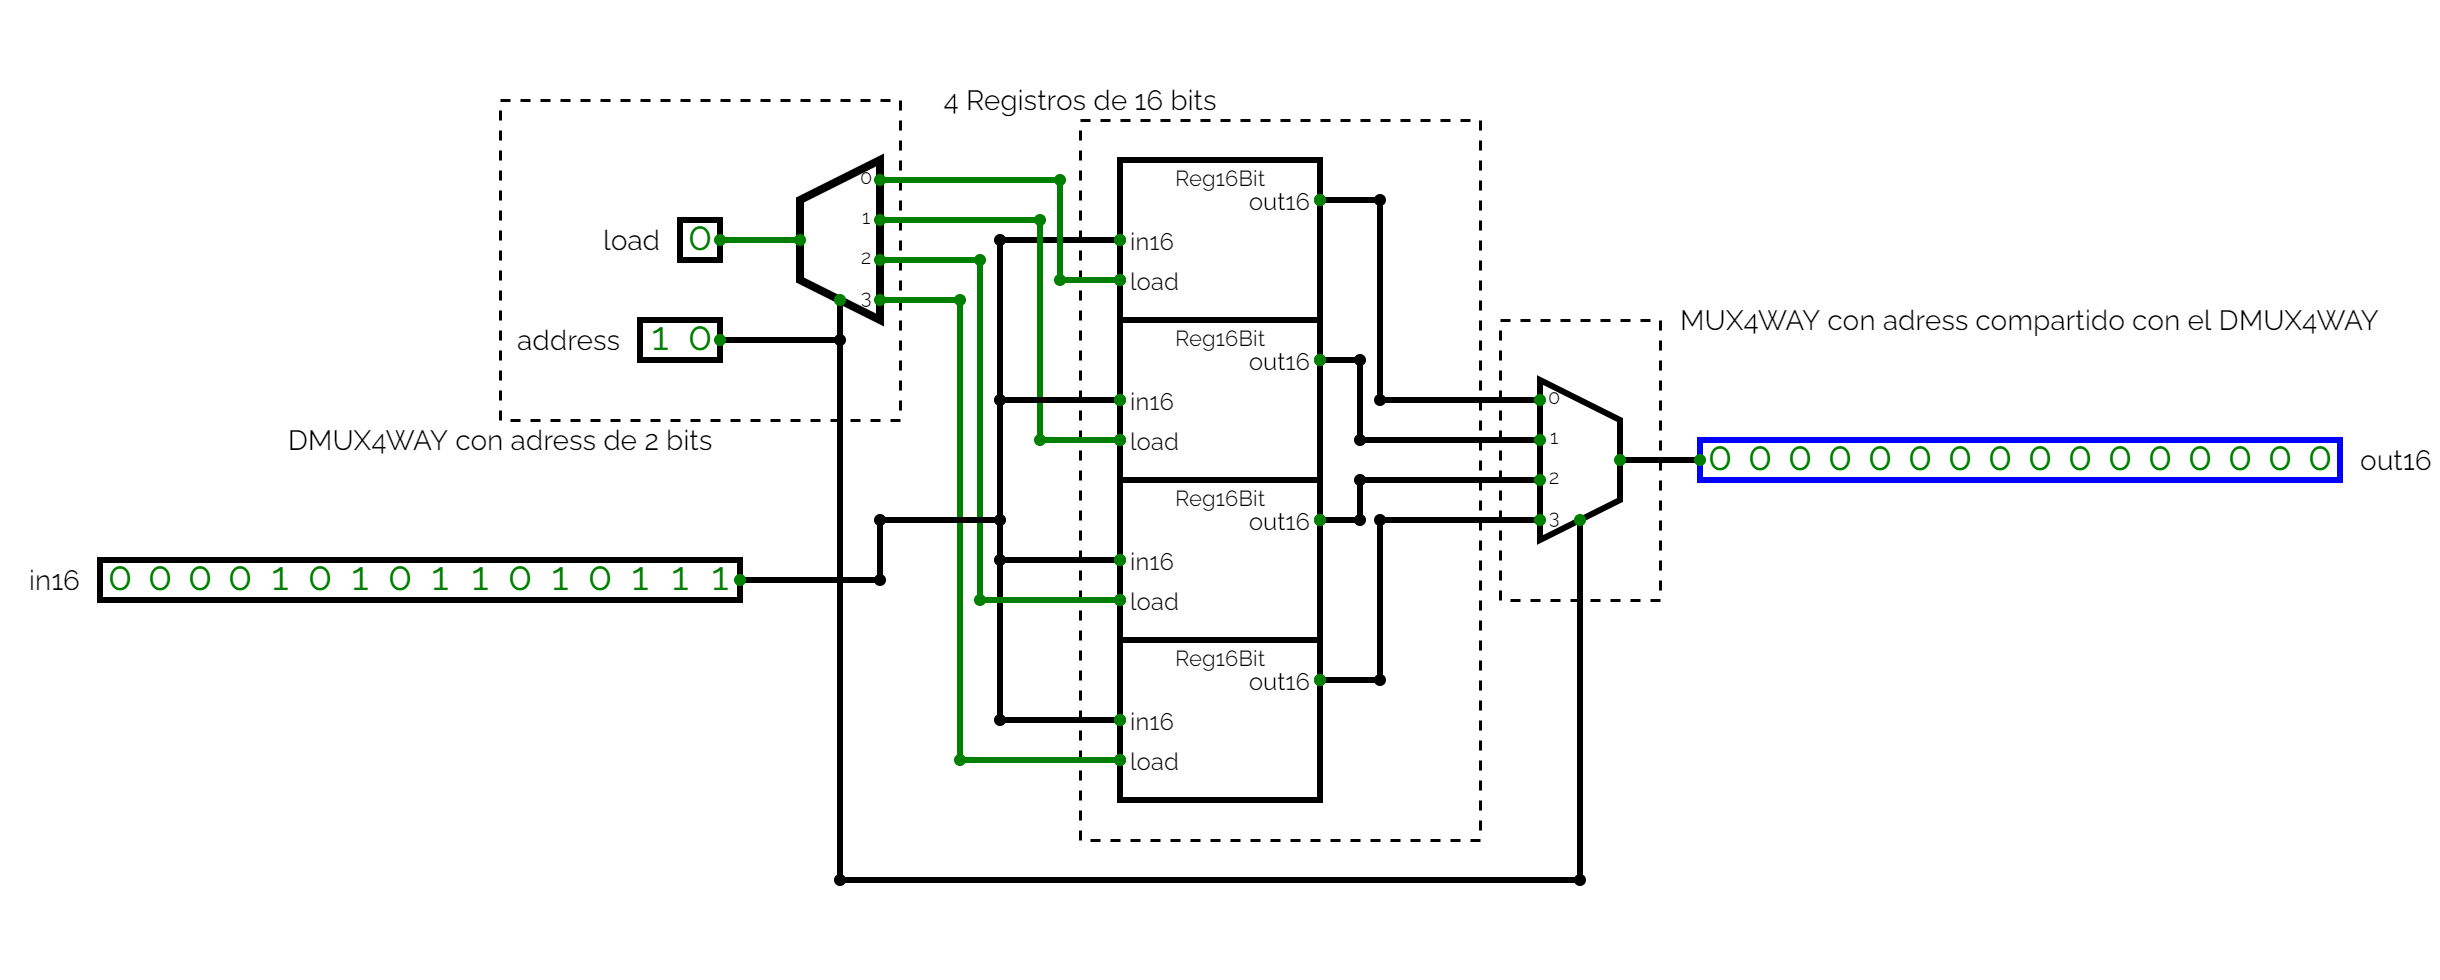
\includegraphics[width=0.75\linewidth]{RAM/RAM_int}
		\caption{Circuito interior de RAM4}
		\label{fig:ramint}
	\end{figure}

Con 2 RAM4, se puede componer una RAM8.
	\begin{figure}[H]
		\centering
		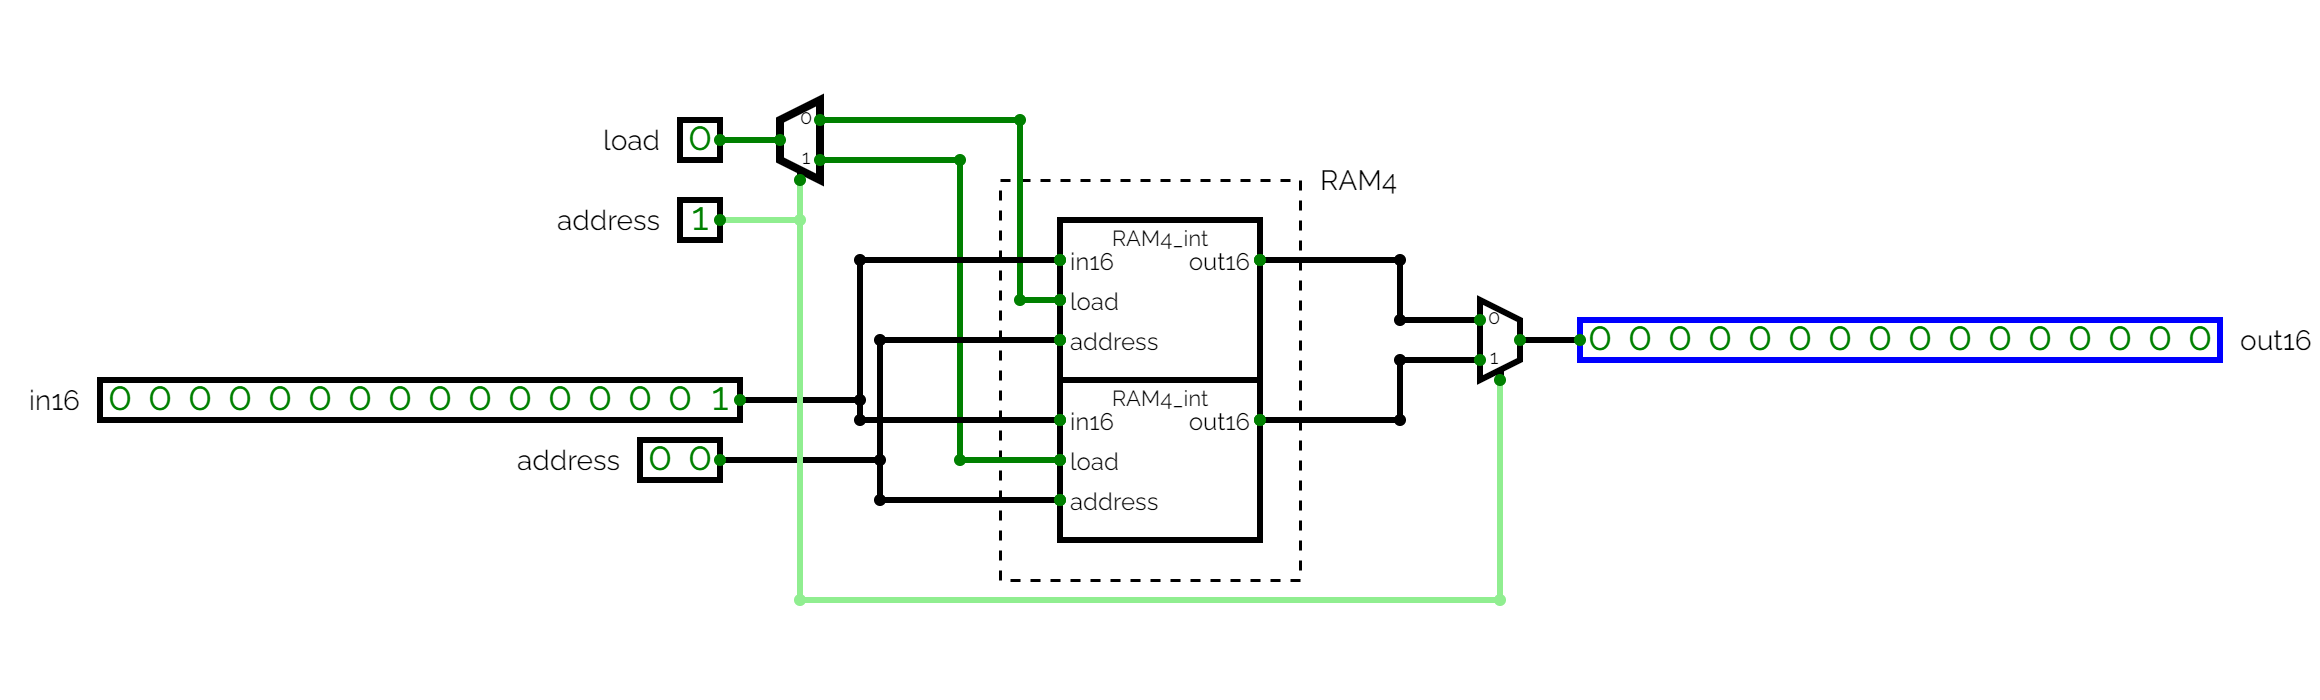
\includegraphics[width=0.75\linewidth]{RAM/RAM8_int}
		\caption{Circuito interior de RAM8}
		\label{fig:ram8int}
	\end{figure}


	\begin{figure}[H]
		\centering
		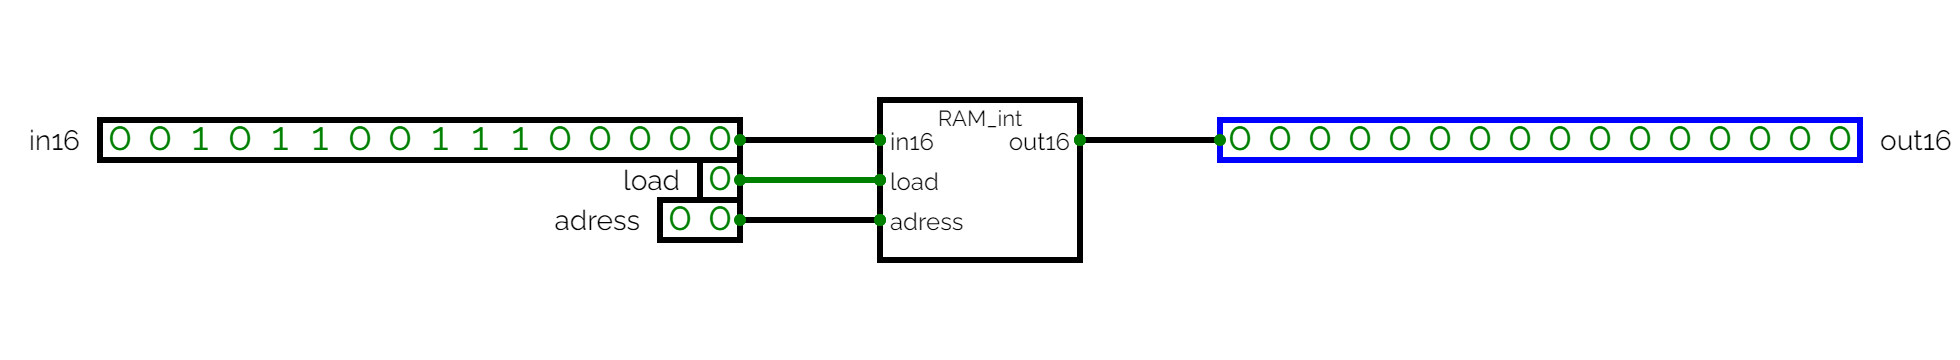
\includegraphics[width=0.75\linewidth]{RAM/RAM_EXT}
		\caption{Circuito exterior de RAM8}
		\label{fig:ramext}
	\end{figure}


\subsection{Implementación HDL}
		\begin{figure}[H]
			\centering
			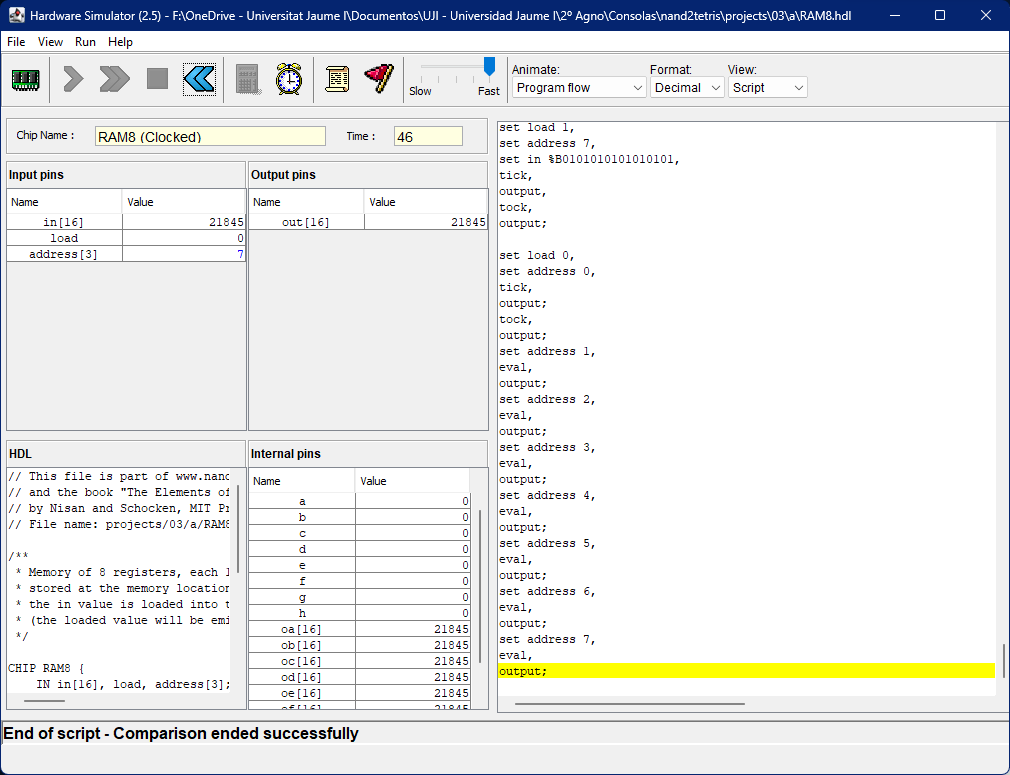
\includegraphics[width=0.75\linewidth]{RAM/ram8_hdl}
			\caption{Implementación en Hardware Simulator de RAM8}
			\label{fig:ram8hdl}
		\end{figure}

		\subsubsection{Archivo .HDL}
			\begin{lstlisting}
	CHIP RAM8 {
		IN in[16], load, address[3];
		OUT out[16];

		PARTS:
		DMux8Way(in=load,sel=address,a=a,b=b,c=c,d=d,e=e,f=f,g=g,h=h);

		Register(in=in,load=a,out=oa);
		Register(in=in,load=b,out=ob);
		Register(in=in,load=c,out=oc);
		Register(in=in,load=d,out=od);
		Register(in=in,load=e,out=oe);
		Register(in=in,load=f,out=of);
		Register(in=in,load=g,out=og);
		Register(in=in,load=h,out=oh);

		Mux8Way16(a=oa,b=ob,c=oc,d=od,e=oe,f=of,g=og,h=oh,sel=address,out=out);
	}
			\end{lstlisting}


\newpage
%%%%%%%%%%%%%%%%%%%%%%%%%%%%%%%%%%%%%%%%%%%%%%%%%%%%%%%%%%%%%%%%%%%%%%%%%%
%%%%%%%%%%%%%%%%%%%%%%%%%%%%%%%%%%%%%%%%%%%%%%%%%%%%%%%%%%%%%%%%%%%%%%%%%%
\printbibliography[heading=bibintoc]
\end{document}
